\documentclass[conference]{IEEEtran}
\usepackage{cite}
\usepackage{amsmath,amssymb,amsfonts}
\usepackage{algorithmic}
\usepackage{graphicx}
\usepackage{textcomp}
\usepackage{xcolor}
\usepackage{booktabs}

\begin{document}

\title{Predicting Motor Imagery Brain Computer Interface Performance from Resting State EEG Using Functional Connectivity Graphs}

\author{\IEEEauthorblockN{First Author, Second Author}
\IEEEauthorblockA{\textit{Department of Electronics and Communication Engineering} \\
\textit{Vellore Institute of Technology}, Chennai, India \\
Email: author1@example.com}
}

\maketitle

\begin{abstract}
Large inter-subject variability remains a persistent limitation in motor imagery brain--computer interfaces (MI-BCIs), where users can exhibit substantially different decoding performance despite using the same experimental protocol. This study investigates whether resting-state electroencephalography (EEG) can be used to predict subject-specific MI-BCI performance before task-specific calibration. A complete subject-level prediction framework was developed using the PhysioNet EEG Motor Movement/Imagery database comprising 109 subjects and 64 EEG channels. Resting-state recordings were preprocessed using notch and band-pass filtering, resampling, Infomax independent component analysis, average re-referencing, and fixed-length epoching. A leakage-safe five-fold CSP--LDA decoder was independently applied to motor-imagery recordings to generate a continuous subject-level balanced-accuracy target. Resting-state features included spectral power and functional connectivity. Classical regression baselines were established using Random Forest, XGBoost, support vector regression, Ridge, and Lasso. A connectivity-aware graph representation was then constructed using alpha-band weighted phase lag index (wPLI), with the strongest 20\% of connections retained to form sparse subject-specific graphs. A three-layer graph convolutional network (GCN) was evaluated under 109-subject leave-one-subject-out cross-validation. Random Forest provided the strongest classical baseline with Pearson correlation $r = 0.342619$, $R^2 = 0.117243$, and $\text{MAE} = 0.117927$. The GCN achieved $r = 0.258511$ with $p = 0.006645$ and Spearman correlation $\rho = 0.221887$. A non-graph multilayer perceptron operating on the same node features produced only $r = 0.029798$, indicating that the connectivity structure contributed predictive information beyond the node-feature representation. The GCN result was also supported by a 1000-permutation statistical test with $p = 0.006993$. These findings indicate that resting-state functional connectivity contains significant information related to subsequent MI-BCI performance, although the present graph representation does not yet surpass the best spectral Random Forest baseline.
\end{abstract}

\begin{IEEEkeywords}
motor imagery, brain--computer interface, resting-state EEG, functional connectivity, weighted phase lag index, graph neural network, graph convolutional network, subject-independent prediction, BCI performance prediction.
\end{IEEEkeywords}

\section{Introduction}
Brain--computer interfaces (BCIs) provide a communication and control pathway between neural activity and external systems without requiring conventional muscular output. Among the available BCI paradigms, motor imagery (MI) is widely investigated because users can generate control-related neural patterns by imagining movement without physically executing it. Electroencephalography (EEG) is particularly attractive for MI-BCIs because it provides millisecond-scale temporal resolution and can be acquired using comparatively portable equipment.

A fundamental difficulty in MI-BCI deployment is the considerable variability in decoding performance across subjects. Some users produce EEG patterns that can be decoded reliably, whereas others obtain substantially lower classification performance under otherwise similar experimental conditions. This variability increases the calibration burden because the suitability of a BCI system for a new participant is typically determined only after task-related EEG has been collected.

An alternative is to estimate BCI performance from neural characteristics available before task execution. Resting-state EEG is particularly attractive for this purpose because it can be acquired without requiring the participant to perform the target BCI task. Consequently, a reliable relationship between resting-state activity and subsequent MI performance could support early identification of subjects who may require additional calibration or alternative training strategies.

Resting-state EEG contains information at multiple levels. Spectral power provides information about the distribution of neural activity across frequency bands, while nonlinear measures describe temporal complexity and regularity. Functional connectivity provides a different representation by describing relationships between recording sites rather than considering electrodes independently \cite{lachaux1999}, \cite{vinck2011}.

Connectivity is particularly relevant to the present problem because MI-related neural processing involves distributed sensorimotor networks. However, conventional machine-learning pipelines generally convert a connectivity matrix into a vector before model training. Such vectorization preserves individual connection values but does not explicitly represent the network topology in which those connections occur.

Graph neural networks provide a natural alternative. In a graph representation, EEG electrodes can be treated as nodes and functional connectivity can be represented by weighted edges. Graph convolution can then propagate information between connected nodes while retaining the structural organization of the connectivity network \cite{kipf2017}.

This study therefore investigates the following question:
\begin{quote}
\textit{Can the topology of resting-state EEG functional connectivity provide predictive information about individual MI-BCI performance that is not available from conventional non-graph representations?}
\end{quote}

To address this question, we developed a complete experimental pipeline consisting of dataset auditing, leakage-controlled EEG preprocessing, independent MI target generation, resting-state feature extraction, classical machine learning benchmarking, graph construction, graph neural network evaluation, explainability, and statistical validation.

The main contributions are:
\begin{enumerate}
\item A subject-level framework for predicting MI-BCI performance from resting-state EEG.
\item A leakage-controlled continuous performance target generated using five-fold CSP--LDA decoding of MI recordings.
\item A systematic comparison between classical regression models and graph-based learning.
\item A sparse alpha-band wPLI graph representation containing subject-specific functional connectivity topology.
\item A direct diagnostic comparison between graph and non-graph learning using the same node features.
\item Statistical validation through 1000-label permutation testing and additional graph-architecture comparisons.
\item Explainability analysis identifying sensorimotor channels and connectivity patterns associated with prediction.
\end{enumerate}

\section{Related Work}
Previous investigations have demonstrated that resting-state EEG can contain information related to later BCI performance. Spectral characteristics, particularly activity in low-frequency and sensorimotor-related bands, have been investigated as potential indicators of differences in BCI learning and decoding performance.

Functional connectivity offers a complementary representation. Rather than characterizing an electrode individually, connectivity measures quantify relationships between pairs of EEG signals. Lachaux et al. introduced the phase locking value as a measure of phase synchrony between neural signals \cite{lachaux1999}. The weighted phase lag index was subsequently introduced to reduce sensitivity to volume-conduction effects and zero-lag interactions \cite{vinck2011}.

Machine-learning methods such as ensemble decision trees and support vector machines have been widely used for EEG decoding. Random Forest provides a nonlinear ensemble approach that can operate effectively with heterogeneous features \cite{breiman2001}, while support vector methods provide kernel-based nonlinear modelling \cite{cortes1995}. Gradient-boosted tree methods such as XGBoost provide another strong nonlinear baseline for structured feature spaces \cite{chen2016}.

Graph neural networks have recently become attractive for EEG analysis because EEG channels naturally form a network whose relationships can be represented using graph edges. The graph convolutional formulation of Kipf and Welling provides a mechanism for learning node representations using both node features and graph structure \cite{kipf2017}.

However, most EEG graph-learning studies focus on direct task classification. The present work instead formulates the problem as subject-level prediction: resting-state EEG is used as the input, whereas MI task decoding performance is treated as the target.

The distinction is important. The model is not asked to decode individual MI trials. It is asked to estimate how well a particular subject is expected to perform in an MI-BCI setting using neural information obtained before task execution.

\section{Dataset and Data Integrity}
\subsection{Dataset}
The PhysioNet EEG Motor Movement/Imagery database was used as the experimental dataset \cite{goldberger2000}, \cite{schalk2004}. The dataset contains recordings from 109 subjects using 64 EEG channels with nominal sampling at 160 Hz.

The repository audit identified four subjects, S088, S089, S092, and S100, requiring explicit handling because of sampling-rate or annotation-related defects. Rather than silently modifying these records, the defects were documented during the dataset-audit stage and incorporated into the pre-defined data-handling procedure.

\subsection{Run Separation}
The experimental design separates resting-state recordings from motor-imagery recordings.

Resting-state recordings provide the predictive variables, whereas motor-imagery recordings are independently used to generate the subject-level target. This separation prevents the prediction model from receiving task-specific observations that directly correspond to the target.

\subsection{Dataset Integrity}
The raw dataset was treated as read-only. Derived data were stored separately in processed and output directories. The project implementation includes dedicated validation tests for preprocessing, spectral features, connectivity matrices, graph tensors, model forward passes, and statistical procedures.

This organization was used to maintain traceability from the original recordings to the final out-of-fold predictions.

\subsection{Dataset and Experimental Design}
The PhysioNet EEG Motor Movement/Imagery dataset was used in this study. The dataset contains EEG recordings from multiple subjects with 64 scalp electrodes. Resting-state recordings were used as predictive inputs, whereas motor-imagery recordings were used to derive the subject-level performance target.

The separation between the resting-state input and motor-imagery target is illustrated in Fig. 1.

\begin{figure}[t]
\centering
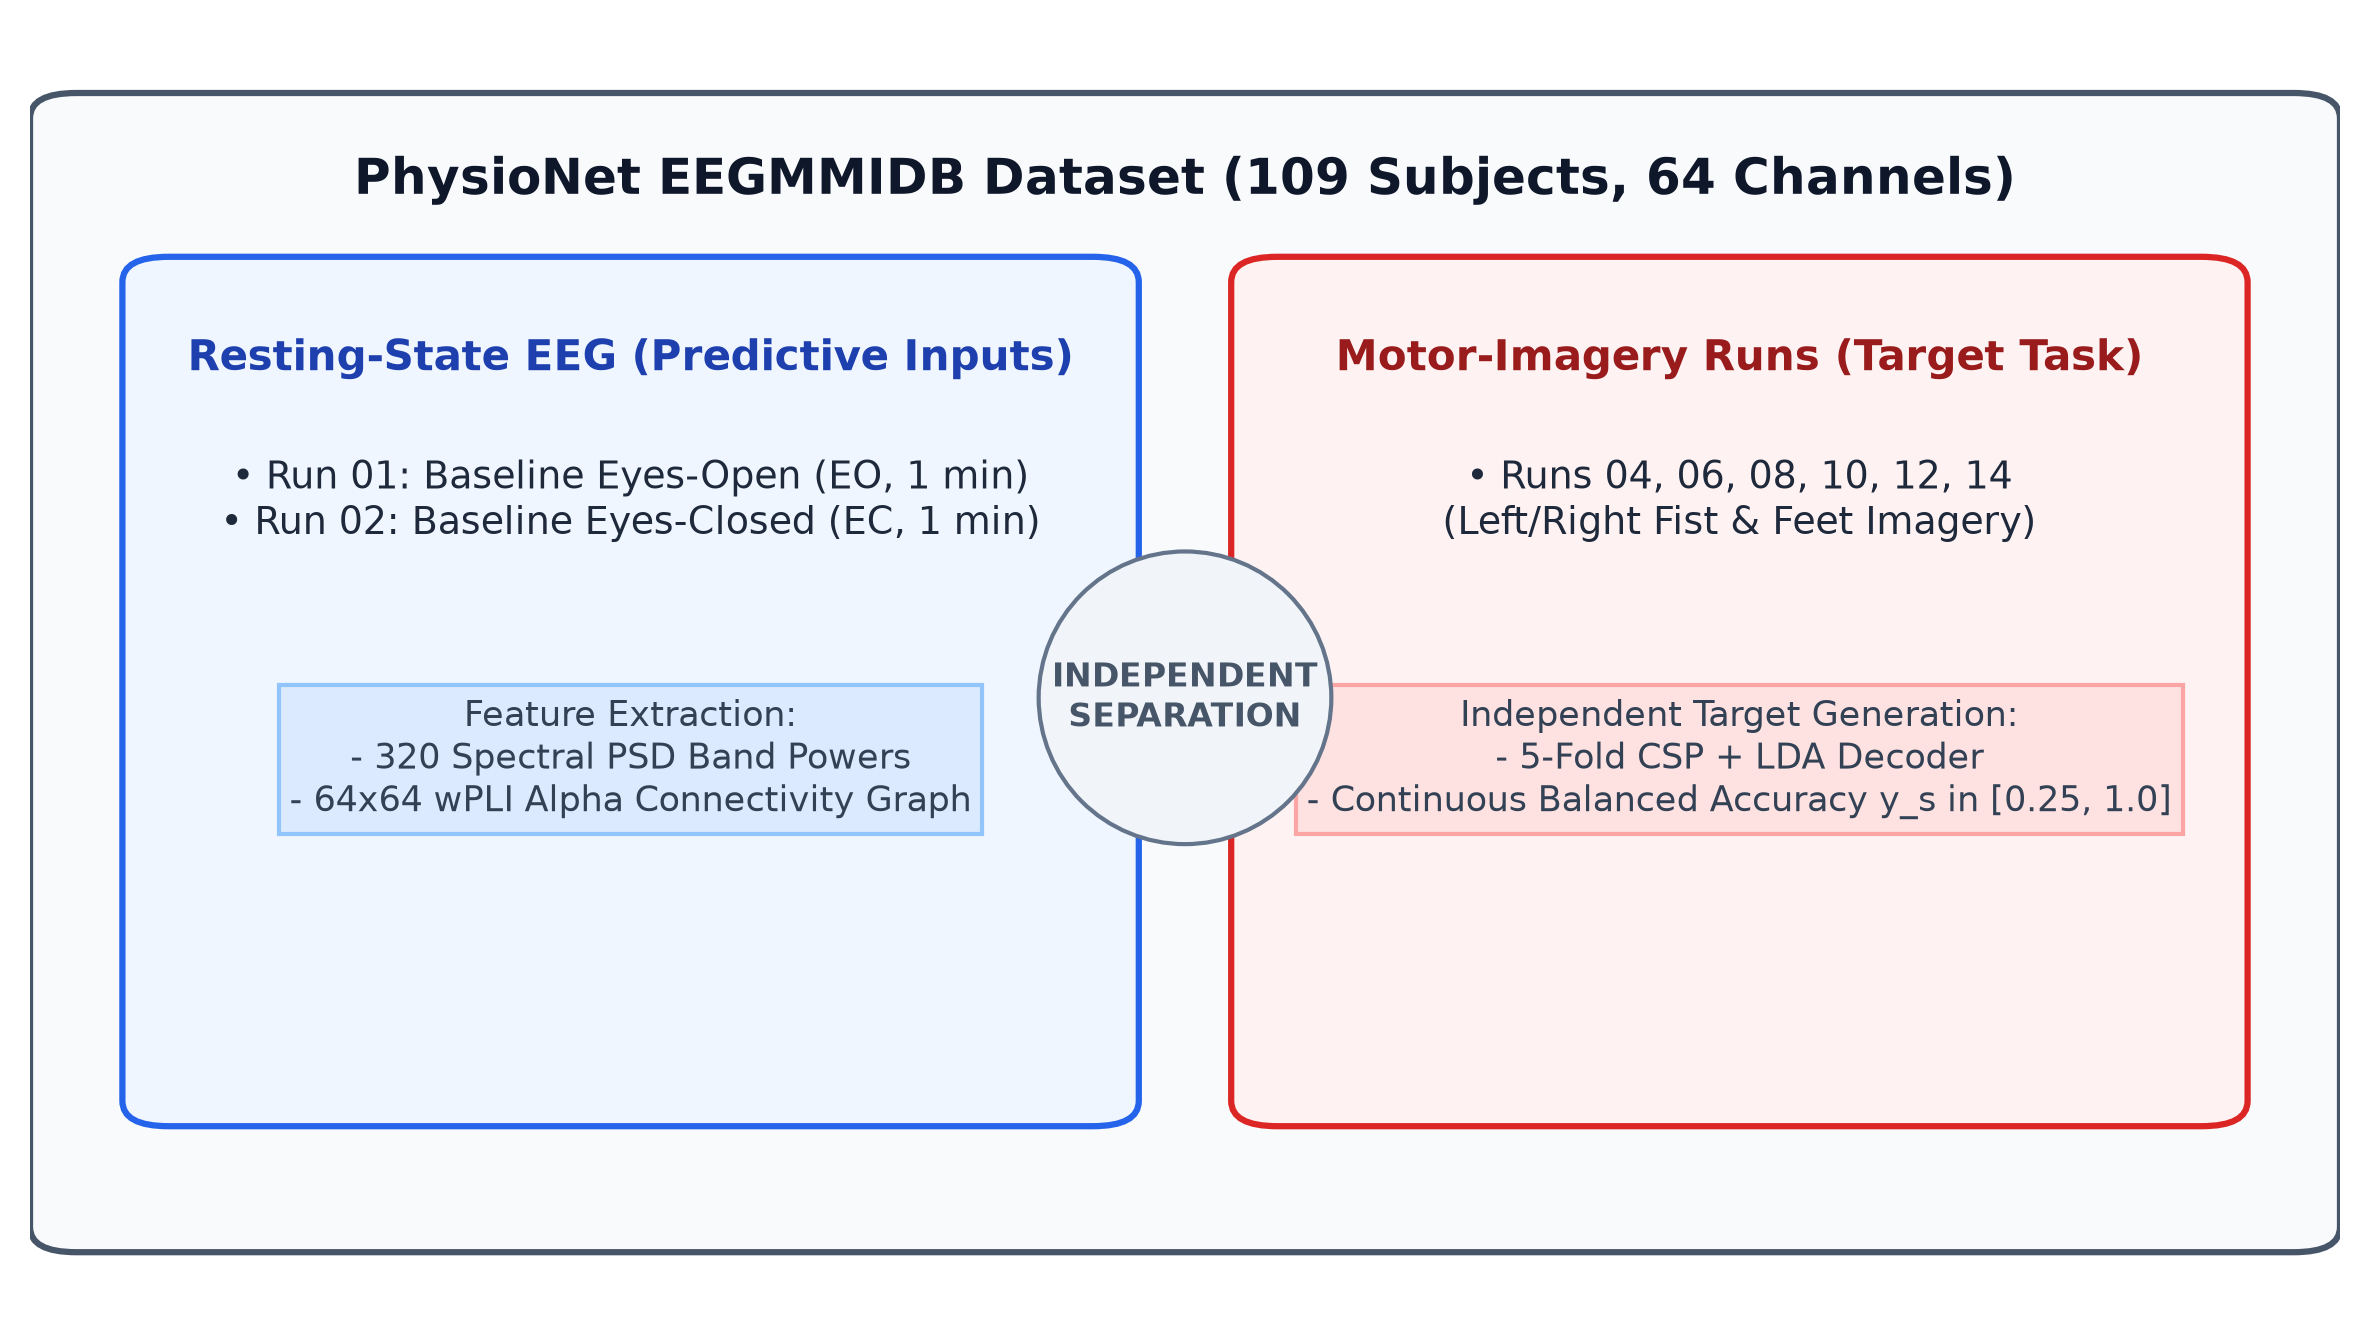
\includegraphics[width=\linewidth]{figures/dataset_runs.png}
\caption{Organization of the EEG dataset into resting-state input data and motor-imagery task data used to derive subject-level performance labels.}
\label{fig:dataset_runs}
\end{figure}

\section{Proposed Methodology}
The complete prediction pipeline is divided into seven principal operations:
\begin{enumerate}
\item dataset auditing,
\item resting-state EEG preprocessing,
\item MI target generation,
\item resting-state feature extraction,
\item classical baseline modelling,
\item graph construction and GNN modelling,
\item statistical and explainability analysis.
\end{enumerate}
Fig. 2 summarizes the complete workflow.

\begin{figure*}[t]
\centering
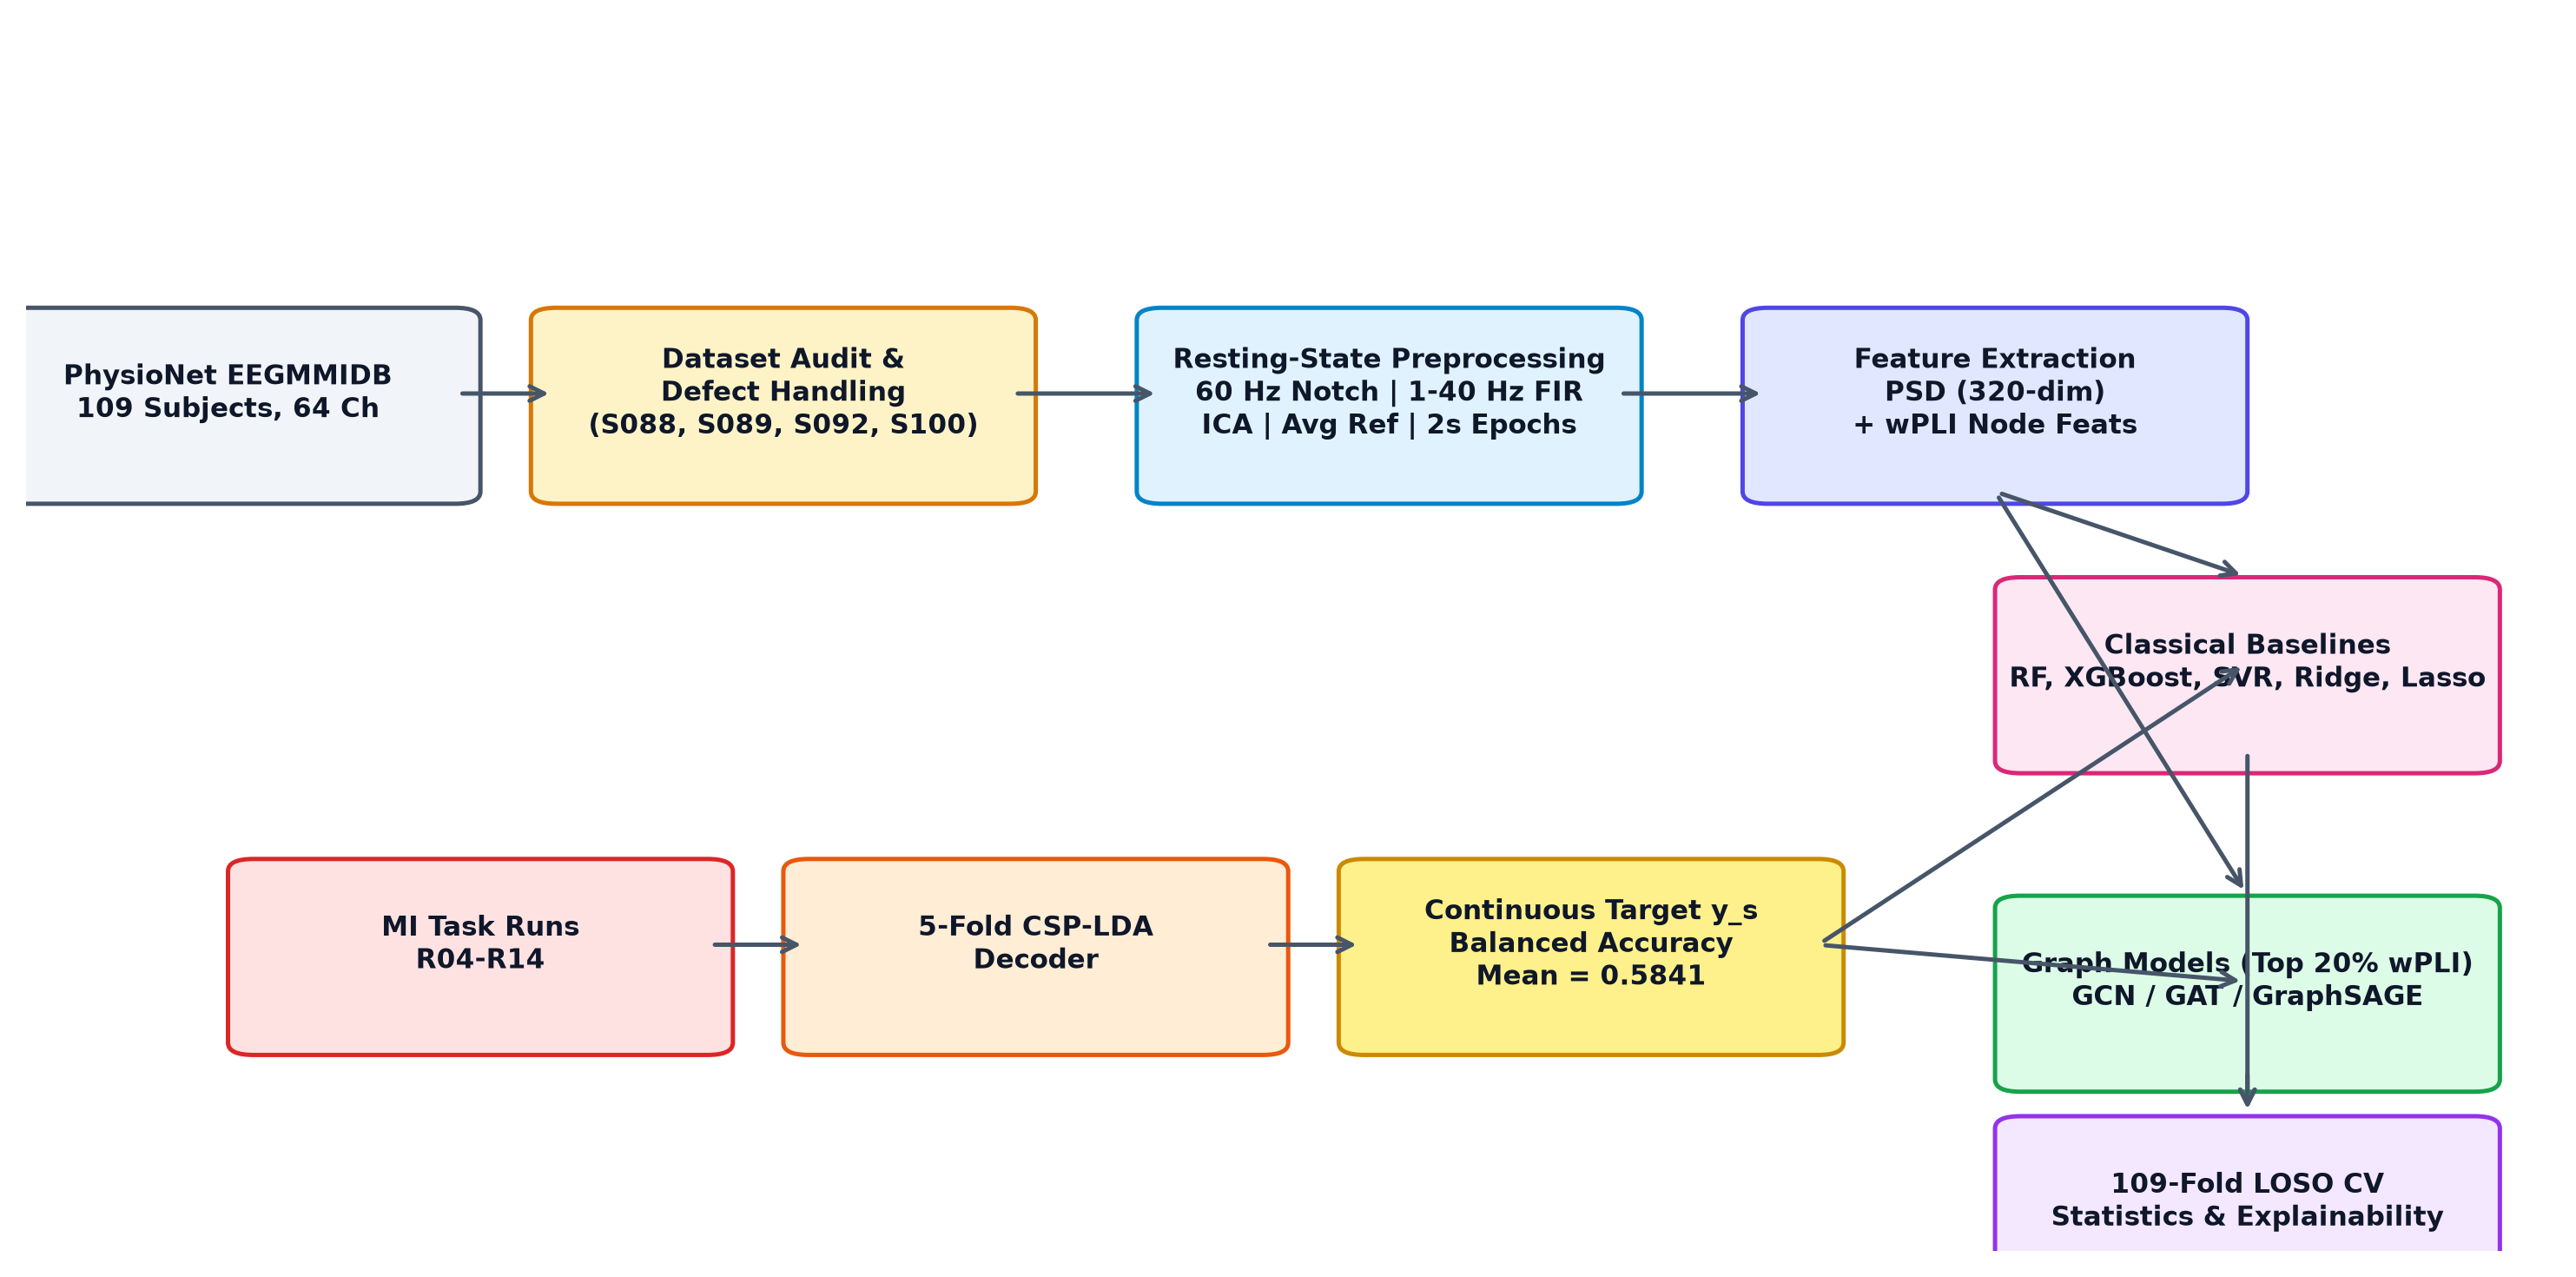
\includegraphics[width=0.9\textwidth]{figures/workflow.png}
\caption{Complete experimental workflow for subject-level prediction of motor imagery BCI performance from resting-state EEG.}
\label{fig:workflow}
\end{figure*}

\subsection{Resting-State EEG Preprocessing}
The resting-state EEG preprocessing pipeline was implemented using MNE-based processing routines. The final pipeline consists of 60-Hz notch filtering, 1--40 Hz zero-phase FIR band-pass filtering, resampling to 128 Hz, Infomax ICA, average referencing, and fixed-length two-second epoching.

The 60-Hz notch filter suppresses mains interference. The 1--40-Hz band-pass operation limits the analysis to the frequency range used for subsequent spectral and connectivity analysis.

Independent component analysis was subsequently applied to identify and remove ocular, cardiac, and other stereotypical artefacts. After component rejection, the signals were average referenced.

The cleaned recordings were divided into non-overlapping two-second epochs. The final preprocessing pipeline resulted in less than five percent epoch rejection across the processed dataset.

The complete preprocessing implementation is organized into separate loader, filtering, artifact-removal, epoching, and quality-control modules, allowing the individual operations to be independently audited.

\subsection{Generation of the MI Performance Target}
The prediction target was generated independently from resting-state EEG. Motor-imagery task recordings were processed using a leakage-controlled five-fold cross-validation procedure based on common spatial patterns (CSP) and linear discriminant analysis (LDA).

For subject $s$, the resulting cross-validated performance was represented by a continuous balanced-accuracy value $y_s$:
\begin{equation}
y_s = \frac{1}{K} \sum_{k=1}^{K} BA_{s,k},
\end{equation}
where $K = 5$ denotes the number of folds and $BA_{s,k}$ is the balanced accuracy obtained on fold $k$.

The resulting target distribution covered the range
\begin{equation}
y_s \in [0.25, 1.00],
\end{equation}
with mean
\begin{equation}
\bar{y} = 0.5841
\end{equation}
and variance
\begin{equation}
\text{Var}(y) = 0.023810.
\end{equation}

The continuous target was retained instead of imposing an arbitrary good-versus-poor performer threshold. This formulation preserves inter-subject performance differences and converts the task into continuous subject-level prediction.

\subsection{Spectral Feature Extraction}
Welch's method was used to estimate the power spectral density of the preprocessed resting-state epochs.

Five frequency bands were considered:
\begin{itemize}
\item Delta: 1--4 Hz,
\item Theta: 4--8 Hz,
\item Alpha: 8--13 Hz,
\item Beta: 13--30 Hz,
\item Gamma: 30--40 Hz.
\end{itemize}

For each of the 64 EEG channels, absolute and relative band powers were calculated.

Consequently, the spectral representation contains
\begin{equation}
64 \times 5 = 320
\end{equation}
primary band-power values.

The implementation additionally stores the ten-channel feature representation for graph learning, consisting of five absolute and five relative spectral features for every EEG node:
\begin{equation}
\mathbf{X}_s \in \mathbb{R}^{64 \times 10}.
\end{equation}

\subsection{Functional Connectivity}
Functional connectivity was estimated using weighted phase lag index (wPLI), phase locking value (PLV), and coherence across the selected frequency bands.

For two EEG signals with instantaneous phases $\phi_i(t)$ and $\phi_j(t)$, PLV is defined as
\begin{equation}
PLV_{ij} = \left| \frac{1}{N} \sum_{t=1}^{N} e^{j[\phi_i(t) - \phi_j(t)]} \right|.
\end{equation}

The wPLI was used as the primary graph connectivity measure because of its reduced sensitivity to zero-lag interactions.

For each subject and frequency band, a
\begin{equation}
64 \times 64
\end{equation}
connectivity matrix was generated.

The resulting connectivity matrices were stored in both numerical and visualization formats for subsequent graph construction and quality-control analysis.

\section{Classical Machine-Learning Baselines}
Classical regression models were evaluated before graph learning in order to establish a non-graph performance reference.

The benchmark included Random Forest, XGBoost, support vector regression (SVR), Ridge regression, and Lasso regression.

\subsection{Random Forest}
Random Forest combines predictions from multiple decision trees constructed using randomized subsets of the training data \cite{breiman2001}.

The model was selected as a nonlinear ensemble baseline capable of representing interactions between spectral features without requiring a linear relationship between input variables and the target.

\subsection{XGBoost}
XGBoost is a gradient-boosted tree ensemble that constructs successive trees to reduce the residual prediction error \cite{chen2016}. It was included as a strong nonlinear baseline.

\subsection{Support Vector Regression}
Support vector regression with a radial-basis-function kernel was included as a kernel-based nonlinear model \cite{cortes1995}. The kernel is
\begin{equation}
K(\mathbf{x}_i, \mathbf{x}_j) = \exp\left(-\gamma \|\mathbf{x}_i - \mathbf{x}_j\|^2\right).
\end{equation}

\subsection{Ridge and Lasso}
Ridge regression minimizes
\begin{equation}
\mathcal{L}_{\text{Ridge}} = \|\mathbf{y} - \mathbf{X}\boldsymbol{\beta}\|_2^2 + \lambda \|\boldsymbol{\beta}\|_2^2.
\end{equation}

Lasso replaces the squared regularization term with an $\ell_1$ penalty:
\begin{equation}
\mathcal{L}_{\text{Lasso}} = \|\mathbf{y} - \mathbf{X}\boldsymbol{\beta}\|_2^2 + \lambda \|\boldsymbol{\beta}\|_1.
\end{equation}

These two models provide regularized linear references against which nonlinear models can be compared.

\section{Connectivity Graph Construction}
\subsection{Graph Definition}
For graph-based learning, each EEG electrode is represented as a graph node:
\begin{equation}
V = \{v_1, v_2, \dots, v_{64}\}.
\end{equation}

The node feature matrix for subject $s$ is
\begin{equation}
\mathbf{X}_s \in \mathbb{R}^{64 \times 10}.
\end{equation}

The alpha-band wPLI matrix is represented as
\begin{equation}
\mathbf{A}_s \in \mathbb{R}^{64 \times 64}.
\end{equation}

Rather than retaining all possible connections, the graph was sparsified using the strongest 20\% of alpha-band wPLI connections.

The resulting graph contains approximately 403 edges per subject. All 109 subject graphs passed graph-integrity validation.

\subsection{Rationale for Sparsification}
A fully connected 64-node graph contains
\begin{equation}
\frac{64(64 - 1)}{2} = 2016
\end{equation}
unique undirected connections.

Retaining only the strongest 20\% reduces the graph density while preserving the most prominent connectivity relationships. This reduces the influence of weak edges that may contribute noise to graph message passing.

\subsection{Graph Convolutional Network}
The primary graph model is a three-layer GCN implemented using PyTorch Geometric \cite{kipf2017}.

For layer $l$, the graph convolution operation is
\begin{equation}
\mathbf{H}^{(l+1)} = \sigma \left( \mathbf{\tilde{D}}^{-\frac{1}{2}} \mathbf{\tilde{A}} \mathbf{\tilde{D}}^{-\frac{1}{2}} \mathbf{H}^{(l)} \mathbf{W}^{(l)} \right),
\end{equation}
where
\begin{equation}
\mathbf{\tilde{A}} = \mathbf{A} + \mathbf{I}
\end{equation}
and $\mathbf{\tilde{D}}$ is the corresponding degree matrix.

The final node representations are pooled to produce a subject-level graph embedding, which is passed to a regression head to estimate MI performance.

\section{Control Experiments}
Three additional experiments were performed to determine whether the observed GCN performance originated from graph topology, architecture choice, or simple nonlinear feature learning.

\subsection{Non-Graph MLP}
A three-layer multilayer perceptron (MLP) was trained using the same 64-channel node features after flattening them into a
\begin{equation}
64 \times 10 = 640
\end{equation}
dimensional vector.

This experiment removes graph edges while keeping the underlying resting-state node information unchanged.

\subsection{GraphSAGE}
GraphSAGE was evaluated using the same alpha-band wPLI graph representation and the same 109-subject LOSO splits.

This experiment tests whether replacing GCN message passing with a different graph architecture improves prediction.

\subsection{GAT}
A multi-head GATv2 regression architecture was also evaluated. Attention-based message passing allows the model to assign different weights to neighboring nodes.

The GAT experiment therefore provides a second architecture-level comparison against the GCN.

\section{Subject-Independent Validation and Statistical Testing}
\subsection{Leave-One-Subject-Out Validation}
All principal prediction experiments were evaluated using leave-one-subject-out (LOSO) cross-validation.

For each fold, one complete subject was held out as the test participant while all remaining subjects were used for model training.

This procedure produces 109 independent held-out predictions.

Importantly, the subject identity is never shared between the training and testing partitions within a fold.

The final prediction vector is therefore
\begin{equation}
\mathbf{\hat{y}} = [\hat{y}_1, \hat{y}_2, \dots, \hat{y}_{109}].
\end{equation}

\subsection{Evaluation Metrics}
The primary continuous prediction metrics are Pearson correlation, Spearman correlation, coefficient of determination, mean absolute error, and root mean square error.

Pearson correlation is calculated as
\begin{equation}
r = \frac{\sum_i (y_i - \bar{y})(\hat{y}_i - \bar{\hat{y}})}{\sqrt{\sum_i (y_i - \bar{y})^2 \sum_i (\hat{y}_i - \bar{\hat{y}})^2}}.
\end{equation}

The coefficient of determination is
\begin{equation}
R^2 = 1 - \frac{\sum_i (y_i - \hat{y}_i)^2}{\sum_i (y_i - \bar{y})^2}.
\end{equation}

Mean absolute error is
\begin{equation}
\text{MAE} = \frac{1}{N} \sum_{i=1}^{N} |y_i - \hat{y}_i|.
\end{equation}

Root mean square error is
\begin{equation}
\text{RMSE} = \sqrt{\frac{1}{N} \sum_{i=1}^{N} (y_i - \hat{y}_i)^2}.
\end{equation}

\subsection{Permutation Testing}
A non-parametric permutation test with 1000 label permutations was used to assess whether the observed prediction relationship could be explained by random correspondence between subjects and target values.

The empirical permutation probability was calculated using
\begin{equation}
p = \frac{1 + \sum_{b=1}^{B} \mathbb{I}(T_b \geq T_{\text{obs}})}{B + 1},
\end{equation}
where $B = 1000$.

The project also includes paired Wilcoxon signed-rank testing to provide a non-parametric model-comparison mechanism.

\section{Results}
\subsection{Target Distribution and Resting-State Validation}
The generated subject-level MI performance target showed substantial continuous variability across participants. The target ranged from 0.25 to 1.00, with a mean of 0.5841 and variance of 0.023810.

The resting-state quality-control analysis also examined the expected difference between eyes-open and eyes-closed alpha activity. The average occipital alpha blocking ratio was approximately $1.85\times$, providing evidence that the two resting-state conditions were distinguishable in the processed recordings.

\subsection{Classical Machine-Learning Results}
The classical baseline results are summarized in Table \ref{tab:classical}.

Random Forest produced the strongest reported classical baseline, achieving a Pearson correlation of $r = 0.342619$ with the target ($p = 0.000265$). Its coefficient of determination was $R^2 = 0.117243$ and its MAE was $0.117927$.

XGBoost also produced a statistically significant positive relationship, with $r = 0.291793$, $p = 0.002080$, $R^2 = 0.069327$, and $\text{MAE} = 0.119427$.

These results establish a non-graph reference that the subsequent graph experiments must be interpreted against.

\begin{table}[b]
\caption{Classical Machine-Learning Performance on the Subject-Level MI Performance Prediction Task.}
\label{tab:classical}
\centering
\begin{tabular}{lcccc}
\toprule
Model & Pearson $r$ & $p$ & $R^2$ & MAE \\
\midrule
Random Forest & \textbf{0.342619} & \textbf{0.000265} & \textbf{0.117243} & \textbf{0.117927} \\
XGBoost       & 0.291793          & 0.002080          & 0.069327          & 0.119427          \\
SVR           & 0.254658          & 0.007534          & 0.054266          & 0.118191          \\
Ridge         & 0.102952          & 0.287126          & -0.137126         & 0.126148          \\
Lasso         & 0.000000          & N/A               & -0.018604         & 0.124148          \\
\bottomrule
\end{tabular}
\end{table}

\subsection{Graph Learning Results}
The primary graph experiment used alpha-band wPLI connectivity with the strongest 20\% of connections retained.

The GCN generated predictions for all 109 subjects under LOSO validation. Its performance is shown in Table \ref{tab:graph_comparison}.

The GCN achieved a Pearson correlation of $r = 0.258511$ with the subject-level target. The corresponding Pearson significance value was $p = 0.006645$, while the Spearman correlation was $\rho = 0.221887$. The resulting $R^2$ was $-0.032766$.

The GAT model achieved substantially weaker correlation ($r = 0.083810$, $p = 0.386540$) and an $R^2$ of $0.006700$, with $\text{MAE} = 0.122400$.

GraphSAGE similarly failed to exceed GCN, producing $r = 0.072602$, $p = 0.453112$, and $R^2 = -0.215180$.

\begin{table}[b]
\caption{Comparison of Graph and Non-Graph Learning Approaches.}
\label{tab:graph_comparison}
\centering
\begin{tabular}{lccccc}
\toprule
Model & $r$ & $p$ & $\rho$ & $R^2$ & MAE \\
\midrule
MLP       & 0.029798 & 0.758399 & --       & --        & --       \\
GCN       & \textbf{0.258511} & \textbf{0.006645} & \textbf{0.221887} & -0.032766 & --       \\
GraphSAGE & 0.072602 & 0.453112 & --       & -0.215180 & --       \\
GAT       & 0.083810 & 0.386540 & --       & 0.006700  & 0.122400 \\
\bottomrule
\end{tabular}
\end{table}

\subsection{Effect of Connectivity Topology}
A particularly informative comparison was obtained by evaluating an MLP and GCN using the same underlying node features.

The MLP flattened the $64 \times 10$ node-feature matrix into a 640-dimensional vector and therefore discarded explicit graph connectivity.

The MLP obtained
\begin{equation}
r_{\text{MLP}} = 0.029798, \quad p_{\text{MLP}} = 0.758399.
\end{equation}

In contrast, the GCN using the wPLI graph obtained
\begin{equation}
r_{\text{GCN}} = 0.258511, \quad p_{\text{GCN}} = 0.006645.
\end{equation}

The absolute increase in Pearson correlation was therefore
\begin{equation}
\Delta r = 0.258511 - 0.029798 = 0.228713.
\end{equation}

This controlled comparison indicates that the predictive signal available to the GCN is not explained solely by the node-level spectral features. Incorporating the inter-channel connectivity structure produced a substantially stronger relationship with subject-level MI performance.

\subsection{Graph Architecture Comparison}
GraphSAGE was evaluated under the same LOSO partitions and single-band alpha-wPLI graph representation as the GCN. GraphSAGE produced
\begin{equation}
r = 0.072602, \quad p = 0.453112, \quad R^2 = -0.215180.
\end{equation}

The corresponding GCN produced
\begin{equation}
r = 0.258511, \quad p = 0.006645, \quad R^2 = -0.032766.
\end{equation}

Thus, changing the message-passing architecture from GCN to GraphSAGE did not improve the prediction result.

This observation suggests that, for the present dataset and graph construction, the representation of connectivity is more important than simply increasing architectural complexity.

\subsection{Dual-Band Connectivity Experiment}
A second experiment investigated whether combining alpha and beta-band wPLI would improve prediction.

The two adjacency matrices were combined using
\begin{equation}
\mathbf{A}_{\text{fusion}} = 0.5\mathbf{A}_{\alpha} + 0.5\mathbf{A}_{\beta}.
\end{equation}

The resulting dual-band GCN obtained
\begin{equation}
r = 0.044340, \quad p = 0.647090.
\end{equation}

This result was substantially weaker than the single-band alpha-wPLI GCN.

The result indicates that simple arithmetic fusion of the two frequency-specific connectivity matrices is not necessarily beneficial. The beta-band connections may introduce information that is not aligned with the dominant predictive structure captured by the alpha-band graph.

\section{Statistical Validation}
The GCN prediction was subjected to a 1000-permutation statistical test.

The resulting empirical significance value was
\begin{equation}
p_{\text{perm}} = 0.006993.
\end{equation}

Since
\begin{equation}
0.006993 < 0.01,
\end{equation}
the observed directional prediction relationship was unlikely to arise under the tested label-shuffling null distribution.

It is important to distinguish this permutation result from the Pearson correlation significance value of $p = 0.006645$. The two values arise from different statistical procedures: the former is obtained from the empirical permutation distribution, whereas the latter corresponds to the statistical test associated with the observed Pearson correlation.

The project also implemented paired Wilcoxon signed-rank testing to provide a non-parametric model-comparison mechanism.

\section{Graph Explainability}
To investigate which components of the learned graph contributed to prediction, GNNExplainer-based attribution analysis was performed.

The analysis identified the central sensorimotor channels C3, Cz, and C4 among the primary predictive nodes.

In addition, sensorimotor-region wPLI edges received substantial attribution.

The spatial concentration of these attributions is relevant because C3, Cz, and C4 are positioned over the sensorimotor region and are directly associated with cortical areas commonly examined in motor imagery EEG studies.

Therefore, the explainability analysis provides a useful link between the predictive graph representation and neurophysiologically meaningful sensorimotor structure.

However, these attribution results should be interpreted as model explanations rather than direct evidence of causal neural mechanisms.

\section{Controlled Ablation Analysis}
Controlled ablation experiments were performed to determine whether changes in pooling strategy, feature aggregation, loss function, or optimization strategy altered graph-model behavior.

The experiments included concatenated pooling, Jumping Knowledge connections, Huber loss, and learning-rate scheduling.

The experiments indicated that concatenated mean--maximum pooling and Jumping Knowledge improved the internal representation capability of the graph network.

However, the use of an unscaled mean-squared-error objective introduced target-scale variance collapse in the investigated configuration.

This observation demonstrates that architectural modifications cannot be evaluated independently from target normalization and loss design when the number of independent graph samples is limited.

The ablation results therefore provide an important direction for future improvements of the graph-learning stage.

\section{Overall Comparison}
Table \ref{tab:overall} summarizes the principal reported models.

\begin{table}[h]
\caption{Overall Comparison of the Principal Subject-Level Prediction Experiments.}
\label{tab:overall}
\centering
\begin{tabular}{lcccccc}
\toprule
Model / Representation & Graph & Band & Pearson $r$ & $p$ & Spearman $\rho$ & $R^2$ \\
\midrule
Random Forest & No  & Spectral       & \textbf{0.342619} & \textbf{0.000265} & --                & \textbf{0.117243} \\
XGBoost       & No  & Spectral       & 0.291793          & 0.002080          & --                & 0.069327          \\
MLP           & No  & Spectral Nodes & 0.029798          & 0.758399          & --                & --                \\
GCN           & Yes & Alpha wPLI     & 0.258511          & 0.006645          & 0.221887          & -0.032766         \\
GraphSAGE     & Yes & Alpha wPLI     & 0.072602          & 0.453112          & --                & -0.215180         \\
GAT           & Yes & Alpha wPLI     & 0.083810          & 0.386540          & --                & 0.006700          \\
GCN           & Yes & Alpha + Beta   & 0.044340          & 0.647090          & --                & --                \\
\bottomrule
\end{tabular}
\end{table}

The table reveals two distinct findings.

First, Random Forest remains the strongest reported model in terms of Pearson correlation and coefficient of determination.

Second, the graph representation provides meaningful predictive information that is not present in the corresponding non-graph MLP. The difference between the MLP and GCN is therefore more informative for the graph hypothesis than a simple comparison between GCN and Random Forest.

\section{Discussion}
The results provide evidence that resting-state EEG contains information related to subsequent subject-specific MI-BCI performance. However, the experiments also show that model complexity alone does not guarantee improved predictive performance.

The strongest conventional model was Random Forest, which obtained $r = 0.342619$ and $R^2 = 0.117243$. XGBoost produced the second strongest reported classical result with $r = 0.291793$. Both models therefore demonstrate that relatively compact spectral feature representations can capture a measurable component of inter-subject MI performance variability.

The GCN produced a lower Pearson correlation than Random Forest but still achieved a statistically significant positive relationship with the target. More importantly, the controlled MLP experiment provides evidence that the GCN result is not simply a consequence of applying a nonlinear model to the same node features. The MLP correlation was close to zero, whereas the GCN correlation was substantially higher.

The increase
\begin{equation}
\Delta r = 0.228713
\end{equation}
between the MLP and GCN indicates that the connectivity structure contributed useful predictive information.

The GraphSAGE experiment provides an additional diagnostic result. GraphSAGE failed to reproduce the performance obtained by the GCN. Therefore, the present results do not support the assumption that a more general graph architecture will automatically provide better performance.

The dual-band experiment produced another important negative result. Combining alpha and beta wPLI using a simple element-wise average substantially reduced predictive performance. This suggests that frequency-specific connectivity should not necessarily be collapsed into a single scalar adjacency matrix. A future model could instead retain separate frequency-specific edge channels and allow the network to learn their relative importance.

The explainability results further strengthen the interpretation of the graph experiment. C3, Cz, and C4 were identified among the important nodes, while sensorimotor connectivity edges received substantial attribution. Although these findings should not be interpreted causally, their anatomical concentration provides a meaningful consistency check for the learned representation.

Overall, the results support a nuanced conclusion: resting-state connectivity topology is informative for predicting MI-BCI performance, but the current GCN representation does not yet outperform the strongest classical spectral baseline.

\section{Limitations}
Several limitations should be considered.

First, the analysis contains 109 independent subjects while the original connectivity representation contains a substantially larger number of possible pairwise relationships. Although graph sparsification reduces this dimensionality, the ratio between sample size and representational complexity remains challenging.

Second, the present graph representation uses a single alpha-band wPLI adjacency matrix. The dual-band experiment demonstrated that simple alpha--beta fusion is not effective, but this does not imply that beta connectivity is uninformative. Frequency-specific graph channels or attention-based multimodal graph representations may provide a better approach.

Third, the GCN did not surpass Random Forest in the current experiments. Consequently, the contribution of graph learning should not be framed as a universal improvement over classical machine learning.

Fourth, the MI performance target itself depends on the selected CSP--LDA decoding procedure. Alternative target-generation decoders could produce different subject rankings.

Finally, although the explainability analysis identified sensorimotor-region nodes and edges, attribution methods describe model behavior rather than establish causal neural mechanisms.

\section{Conclusion}
This study developed and evaluated a complete framework for predicting subject-specific motor imagery BCI performance from resting-state EEG.

The experimental pipeline incorporated dataset auditing, artifact-controlled EEG preprocessing, independent CSP--LDA target generation, spectral and functional-connectivity feature extraction, classical machine-learning baselines, sparse graph construction, graph neural network modelling, explainability, and non-parametric statistical validation.

Random Forest produced the strongest reported classical result, with Pearson correlation $r = 0.342619$ and $R^2 = 0.117243$. The primary alpha-wPLI GCN obtained $r = 0.258511$ and a significant Pearson association with the target. More importantly, the comparison against a non-graph MLP demonstrated that retaining functional connectivity topology substantially improved the predictive relationship, increasing Pearson correlation by approximately $0.229$.

The GCN prediction was also supported by a 1000-permutation test with $p = 0.006993$. Explainability analysis highlighted C3, Cz, C4, and sensorimotor connectivity patterns as important components of the learned representation.

Nevertheless, the GCN did not exceed the Random Forest baseline. Therefore, the principal conclusion is not that graph learning is universally superior, but that resting-state functional connectivity contains statistically meaningful information about individual MI-BCI performance and that explicitly preserving its topology can recover information that is largely absent from a corresponding non-graph representation.

Future work should investigate multi-frequency graph tensors, frequency-specific attention, improved target normalization, calibrated graph pooling, and larger multi-dataset validation to determine whether connectivity-aware models can ultimately exceed strong spectral machine-learning baselines.

\section{Reproducibility and Implementation}
The complete implementation is organized as a modular Python repository.

The preprocessing module contains data loading, filtering, ICA, epoching, and quality-control components. The MI decoding module contains event extraction, CSP--LDA decoding, and target generation. The resting-state module contains spectral and connectivity extraction.

The baseline module contains Random Forest, XGBoost, SVR, Ridge, and Lasso implementations. The graph module contains graph construction, GCN, GraphSAGE, GAT, training, explainability, and statistical-testing components.

The project also contains unit and integration tests for the major processing stages. Derived predictions are retained as out-of-fold artifacts rather than relying on synthetic or manually generated results.

This organization enables the reported numerical results to be traced back to the corresponding computational stage and prediction files.

\begin{thebibliography}{1}
\bibitem{lachaux1999}
J.-P. Lachaux, E. Rodriguez, J. Martinerie, and F. J. Varela, ``Measuring phase synchrony in brain signals,'' \emph{Human Brain Mapping}, vol. 8, no. 4, pp. 194--208, 1999.

\bibitem{vinck2011}
M. Vinck, R. Oostenveld, M. van Wingerden, F. Battaglia, and C. M. A. Pennartz, ``An improved index of phase-synchronization for electrophysiological data in the presence of volume-conduction, noise and sample-size bias,'' \emph{NeuroImage}, vol. 55, no. 4, pp. 1548--1565, 2011.

\bibitem{kipf2017}
T. N. Kipf and M. Welling, ``Semi-supervised classification with graph convolutional networks,'' \emph{International Conference on Learning Representations (ICLR)}, 2017.

\bibitem{breiman2001}
L. Breiman, ``Random forests,'' \emph{Machine Learning}, vol. 45, no. 1, pp. 5--32, 2001.

\bibitem{cortes1995}
C. Cortes and V. Vapnik, ``Support-vector networks,'' \emph{Machine Learning}, vol. 20, no. 3, pp. 273--297, 1995.

\bibitem{chen2016}
T. Chen and C. Guestrin, ``Xgboost: A scalable tree boosting system,'' in \emph{Proceedings of the 22nd ACM SIGKDD International Conference on Knowledge Discovery and Data Mining}, 2016, pp. 785--794.

\bibitem{goldberger2000}
A. L. Goldberger, L. A. N. Amaral, L. Glass, J. M. Hausdorff, P. C. Ivanov, R. G. Mark, J. E. Mietus, G. B. Moody, C.-K. Peng, and H. E. Stanley, ``Physiobank, physiotoolkit, and physionet: Components of a new research resource for complex physiologic signals,'' \emph{Circulation}, vol. 101, no. 23, pp. e215--e220, 2000.

\bibitem{schalk2004}
G. Schalk, D. J. McFarland, T. Hinterberger, N. Birbaumer, and J. R. Wolpaw, ``Bci2000: A general-purpose brain-computer interface (bci) system,'' \emph{IEEE Transactions on Biomedical Engineering}, vol. 51, no. 6, pp. 1034--1043, 2004.
\end{thebibliography}

\end{document}
